%
% einleitung.tex -- Beispiel-File für die Einleitung
%
% (c) 2020 Prof Dr Andreas Müller, Hochschule Rapperswil
%
% !TEX root = ../../buch.tex
% !TEX encoding = UTF-8
%
%Elektrodynmaik
\tikzset{>=latex} % for LaTeX arrow head
\colorlet{myblue}{black!40!blue}
\colorlet{myred}{black!40!red}
\colorlet{vcol}{green!50!black}
\colorlet{Ecol}{orange!90!black}
\colorlet{EVcol}{orange!80!black!60}
\colorlet{Bcol}{violet!90}

\section{Elektrodynamik\label{section:maxwell:elektrodynmaik}}
\rhead{Elektrodynamik}
In der Elektrodynamik erlauben wir, dass
\[
\frac{\partial f}{\partial t}
\neq
0
\]
für die Funktionen, die wir betrachten, gelten darf.
Das heisst Ladungen dürfen sich nun mit einer beliebigen Geschwindigkeit $\vec{v}$ bewegen und wir berücksichtigen zeitabhängige Skalar- und Vektorfelder.
Bei den statischen Maxwell-Gleichungen fällt auf, dass das elektrische und magnetische Feld keinerlei Abhängigkeiten voneinander haben.
Wie sich später herausstellen wird, ändert sich dies, denn die Zeitabhängigkeit führt dazu, dass sich das elektrische und magnetische Feld gegenseitig beeinflussen.
Daraus folgen einige spannende Tatsachen, auf die wir später noch zu Sprechen kommen.
 
Im folgenden werden wir unseren Raum definieren und bekannte Vektorfelder in ihrer Definition anpassen.

\subsubsection{Der vierdimensionale Raum}
Den Raum in dem wir uns nun bewegen werden, definieren wir als
\begin{equation}
	\Omega
	=
	\begin{pmatrix}
		ct\\
		x\\
		y\\
		z
	\end{pmatrix}
	=
	\Omega^{\mu} \subset \mathbb{R}^4,
\end{equation}
wobei $\Omega^0$ die Zeit $t$ multipliziert mit der Lichtgeschwindigkeit
\[
c
=
\frac{1}{\sqrt{\varepsilon_0\,\mu_0}}
\]
ist.
Damit wir uns später ein wenig Schreibaufwand sparen können, schreiben wir die Ableitungen der Raumkomponenten als
\[
\frac{\partial}{\partial \Omega^{\mu}}
=
\partial^{\mu}.
\]

\subsubsection{4er Gradient}
Der 4er Gradient einer Funktion $f: \mathbb{R}^4 \rightarrow \mathbb{R}$ im Raum $\Omega$ ist von der Form
\[
\renewcommand{\arraystretch}{1.9}
\nabla^\mu f
=
\begin{pmatrix}
	\displaystyle
	\partial^0 f\\
	\displaystyle
	\partial^1 f\\
	\displaystyle
	\partial^2 f\\
	\displaystyle
	\partial^3 f
\end{pmatrix}
=
\begin{pmatrix}
	\displaystyle
	\frac{\partial f}{\partial (ct)}\\
	\displaystyle
	\frac{\partial f}{\partial x}\\
	\displaystyle
	\frac{\partial f}{\partial y}\\
	\displaystyle
	\frac{\partial f}{\partial z}
\end{pmatrix}
=
\begin{pmatrix}
	\displaystyle
	\frac{1}{c}\frac{\partial f}{\partial t}\\
	\displaystyle
	\frac{\partial f}{\partial x}\\
	\displaystyle
	\frac{\partial f}{\partial y}\\
	\displaystyle
	\frac{\partial f}{\partial z}
\end{pmatrix}
=
\begin{pmatrix}
	\displaystyle
	\frac{1}{c}\frac{\partial f}{\partial t}\\
	\displaystyle
	\nabla f
\end{pmatrix}.
\]


\subsubsection{Elektrisches Feld dynamisch}
Das elektrische Feld
\(
\vec{E}: \mathbb{R}^4 \rightarrow \mathbb{R}^3
\)
wird in der Elektrodynamik definiert als
\begin{equation}
	\vec{E}(t,x,y,z)
	=
	- \nabla\varphi(t,x,y,z) - \frac{\partial \vec{A}}{\partial t}(t,x,y,z).
	\label{maxwell:section:definiton_dynamisch_elektrischesFeld}
\end{equation}
Es fällt auf, dass das elektrische Feld, das elektrische Potentialfeld und das magnetische Vektorpotential nun einen vierdimensionalen Inputvektor besitzen, wobei die zusätzliche Dimension die Zeit ist. 

\subsubsection{Magnetisches Feld dynamisch}
Das magnetische Feld
\(
\vec{B}: \mathbb{R}^4 \rightarrow \mathbb{R}^3
\)
wird in der Elektrodynamik ähnlich definiert wie in der Magnetostatik. Nämlich als
\begin{equation}
	\vec{B}(t,x,y,z)
	=
	\nabla \times \vec{A}(t,x,y,z).
	\label{maxwell:section:definition_dynamisch_magnetischesFeld}
\end{equation}
Der Unterschied liegt hier einzig in der zusätzlichen Zeitkomponente im Inputvektor.

\subsection{Dynamische Maxwell-Gleichungen}
Das Ziel dieses Abschnittes ist ein Variationsprinzip zu formulieren, welches uns die Verhaltensgleichungen der Elektrodynamik liefert. 
Wir betrachten nun den luftleeren, vierdimensionalen Raum $\Omega$.
In diesem Raum existieren nun das elektrische Feld $\vec{E}(t,x,y,z)$, das magnetische Feld $\vec{B}(t,x,y,z)$, eine Stromdichte $\vec{\jmath}(t,x,y,z)$ und eine statische Ladungsdichte $\varrho(x,y,z)$.

\subsubsection{Ansatz}
Wir wählen einen ähnlichen Ansatz wie bislang, nämlich ein Integral über die Zeit der Energie im Raum zu minimieren.
Das Integral über die Zeit ist notwendig, da wir über alle Inputgrössen integrieren müssen.
Diese neue Grösse werden wir mit $D$ bezeichnen.
Durch Superponierung unserer bisher gefundenen Energien erhalten wir
\begin{align*}
	D
	&=
	\int_{(ct)_0}^{(ct)_1} W_{\text{tot}}\,d(ct)
	=
	\int_{t_0}^{t_1} \left(W_{\text{e}} - W_{\text{q}} + W_{\text{p}} - W_{\text{m}}\right)c\,dt
	\\
	&= \int_{\Omega} \frac{1}{2}\,\varepsilon_0\,\vec{E}\,^2 - \varphi\,\varrho 
	+ \vec{A}\cdot\vec{\jmath} - \frac{1}{2\mu_0}\vec{B}^2 \,d\Omega.
\end{align*}
Man sieht hier sehr schön, wie die Feldenergie aus dem Term
\[
w_{\text{e}} - w_{\text{m}}
=
\frac{1}{2}\,\varepsilon_0\,\vec{E}^2 - \frac{1}{2\,\mu_0}\vec{B}^2
\]
besteht und die Kopplungsterme 
\(
\varphi\,\varrho
\)
und
\(
\vec{A}\cdot\vec{\jmath}
\)
sind.
Hiermit ist es uns allerdings noch nicht gelungen ein Energiefunktional zu formulieren, welches von der Form
\[
I(f) = \int_{t_0}^{t_1} \int_{z_0}^{z_1} \int_{y_0}^{y_1} \int_{x_0}^{x_1} L(t,x,y,z,f,f_t,f_x,f_y,f_z)\,dx\,dy\,dz\,dt 
\]
ist, weil das elektrische und magnetische Feld von unterschiedlichen Potentialen abhängig sind.

\subsubsection{Elektromagnetisches 4er Potential}
An dieser Stelle führen wir ein neues Vektorfeld ein, welches die Potentiale des elektrischen und magnetischen Feldes beinhaltet.
Dieses neue Vektorfeld heisst elektromagnetisches 4er Potential
\(
A:\mathbb{R}^4 \rightarrow \mathbb{R}^4
\)
und wird als
\begin{equation}
	A
	=
	\begin{pmatrix}
		\varphi / c\\
		A_x\\
		A_y\\
		A_z
	\end{pmatrix}
	=
	A^{\mu},
\end{equation}
definiert, wobei $A_x$, $A_y$, $A_z$ die Komponenten des magnetischen Vektorpotentiales $\vec{A}$ sind.
Mittels dieser Grösse können wir nun das elektrische und magnetische Feld ausdrücken.
Also
\begin{equation}
\frac{1}{c}\, \vec{E}
=
-\frac{1}{c}\, \nabla\,\varphi - \frac{1}{c}\,\frac{\partial \vec{A}}{\partial t}
=
\begin{pmatrix}
	-\partial^1 A^0 - \partial^0 A^1\\
	-\partial^2 A^0 - \partial^0 A^2\\
	-\partial^3 A^0 - \partial^0 A^3
\end{pmatrix}
=
\begin{pmatrix}
	E_x / c\\
	E_y / c\\
	E_z / c
\end{pmatrix}
\end{equation}
und
\begin{equation}
\vec{B}
=
\nabla \times \vec{A}
=
\begin{pmatrix}
	\partial^2 A^3 - \partial^3 A^2\\
	\partial^3 A^1 - \partial^1 A^3\\
	\partial^1 A^2 - \partial^2 A^1
\end{pmatrix}
=
\begin{pmatrix}
	B_x\\
	B_y\\
	B_z
\end{pmatrix}.
\end{equation}
Daraus ergibt sich für die Feldenergiedichten
\[
w_{\text{e}}
=
\frac{1}{2}\underbrace{\varepsilon_0\,c^2}_{\displaystyle=1/\mu_0} \biggl(\left(\partial^0 A^1 + \partial^1 A^0\right)^2 + \left(\partial^0 A^2 + \partial^2 A^0\right)^2 + 
\left(\partial^0 A^3 + \partial^3 A^0\right)^2\biggr)
\]
und 
\[
w_{\text{m}}
=
\frac{1}{2\mu_0}\,\biggl(\left(\partial^2 A^3 - \partial^3 A^2\right)^2 + \left(\partial^3 A^1 - \partial^1 A^3\right)^2 + 
\left(\partial^1 A^2 - \partial^2 A^1\right)^2\biggr).
\]

\subsubsection{4er Stromdichte}
Damit wir nun auch die Kopplungsterme mit dem elektromagnetischen 4er Potential ausdrücken können, führen wir die 4er Stromdichte
\(
J:\mathbb{R}^4 \rightarrow \mathbb{R}^4
\)
ein. Wir definieren sie als
\begin{equation}
J
=
\begin{pmatrix}
	-c\varrho\\
	j_x\\
	j_y\\
	j_z
\end{pmatrix}
=
J^{\mu},
\end{equation}
wobei $j_x$, $j_y$ und $j_z$ die Komponenten der Stromdichte $\vec{\jmath}$ sind.
Somit können wir unsere beiden Kopplungsterme schön kompakt  als
\begin{equation}
	w_{\text{p}} - w_{\text{q}}
	=
	J\cdot A
\end{equation}
schreiben.

\subsubsection{Formulierung der Lagrange-Funktion}
Uns ist es nun gelungen die Grösse $D$ mit einer Funktion und ihren partiellen Ableitungen zu formulieren. Nämlich ist 
\begin{align*}
D
=
\int_{\Omega}
\frac{1}{2\mu_0}\,\biggl(\left(\partial^0 A^1 + \partial^1 A^0\right)^2 + \left(\partial^0 A^2 + \partial^2 A^0\right)^2 + 
\left(\partial^0 A^3 + \partial^3 A^0\right)^2\biggr) \\
-  \frac{1}{2\mu_0}\,\biggl(\left(\partial^2 A^3 - \partial^3 A^2\right)^2 + \left(\partial^3 A^1 - \partial^1 A^3\right)^2 + 
\left(\partial^1 A^2 - \partial^2 A^1\right)^2\biggr)\\
+ J^0 A^0 + J^1 A^1 + J^2 A^2 + J^3 A^3 \,d\Omega
\end{align*}
und somit die Lagrange-Funktion
\begin{align*}
L(\Omega^0,...,\Omega^3, A^0,...,A^3, \partial^0 A^i,...,\partial^3 A^i)
=
\frac{1}{2\mu_0}\,\biggl(\left(\partial^0 A^1 + \partial^1 A^0\right)^2 + \left(\partial^0 A^2 + \partial^2 A^0\right)^2 + 
\left(\partial^0 A^3 + \partial^3 A^0\right)^2\biggr) \\
-  \frac{1}{2\mu_0}\,\biggl(\left(\partial^2 A^3 - \partial^3 A^2\right)^2 + \left(\partial^3 A^1 - \partial^1 A^3\right)^2 + 
\left(\partial^1 A^2 - \partial^2 A^1\right)^2\biggr)\\
+ J^0 A^0 + J^1 A^1 + J^2 A^2 + J^3 A^3.
\end{align*}

\subsubsection{Einsetzen in die Euler-Ostrogradski-Differentialgleichung}
Da unsere Lagrange-Funktion wiederum von einer vektoriellen Grösse abhängig ist, erhalten wir diesmal vier Euler-Ostrogradski-Differentialgleichungen von der Form
\[
\frac{\partial L}{\partial A^i} 
- \frac{\partial}{\partial \Omega^0}\frac{\partial L}{\partial(\partial^0 A^i)}
- \frac{\partial}{\partial \Omega^1}\frac{\partial L}{\partial(\partial^1 A^i)}
- \frac{\partial}{\partial \Omega^2}\frac{\partial L}{\partial(\partial^2 A^i)}
- \frac{\partial}{\partial \Omega^3}\frac{\partial L}{\partial(\partial^3 A^i)}
= 0 \qquad \text{für } i=0,1,2,3 \,.
\]

{\larger\textcircled{\smaller[2]1}} $i = 0$
\[
J^0  -\frac{1}{\mu_0}\,\biggl(\partial^1\underbrace{\left(\partial^0 A^1 + \partial^1 A^0\right)}_{\displaystyle=-E_x/c}
+ \partial^2\underbrace{\left(\partial^0 A^2 + \partial^2 A^0\right)}_{\displaystyle=-E_y/c}
+ \partial^3\underbrace{\left(\partial^0 A^3 + \partial^3 A^0\right)}_{\displaystyle=-E_z/c}\biggr)
=
0
\]

{\larger\textcircled{\smaller[2]2}} $i = 1$
\[
J^1  -\frac{1}{\mu_0}\,\biggl(\partial^0\underbrace{\left(\partial^0 A^1 + \partial^1 A^0\right)}_{\displaystyle=-E_x/c}
+ \underbrace{\partial^2\left(\partial^1 A^2 + \partial^2 A^1\right)
	- \partial^3\left(\partial^3 A^1 + \partial^1 A^3\right)}_{\displaystyle=(\nabla\times\vec{B})_x}\biggr)
=
0
\]

{\larger\textcircled{\smaller[2]3}} $i = 2$
\[
J^2  -\frac{1}{\mu_0}\,\biggl(\partial^0\underbrace{\left(\partial^0 A^2 + \partial^2 A^0\right)}_{\displaystyle=-E_y/c}
+ \underbrace{\partial^3\left(\partial^2 A^3 + \partial^3 A^2\right)
	- \partial^1\left(\partial^1 A^2 + \partial^2 A^1\right)}_{\displaystyle=(\nabla\times\vec{B})_y}\biggr)
=
0
\]

{\larger\textcircled{\smaller[2]4}} $i = 3$
\[
J^3  -\frac{1}{\mu_0}\,\biggl(\partial^0\underbrace{\left(\partial^0 A^3 + \partial^3 A^0\right)}_{\displaystyle=-E_z/c}
+ \underbrace{\partial^1\left(\partial^3 A^1 + \partial^1 A^3\right)
	- \partial^2\left(\partial^2 A^3 + \partial^3 A^2\right)}_{\displaystyle=(\nabla\times\vec{B})_z}\biggr)
=
0
\]
Für $i=0$ resultiert die partielle Differentialgleichung
\begin{align}
-c\varrho + \frac{1}{\mu_0\,c}\,\biggl(\frac{\partial E_x}{\partial x}
+ \frac{\partial E_y}{\partial y} + \frac{\partial E_z}{\partial z}\biggr)
&=
0\\[1em]
\Leftrightarrow \qquad \nabla\cdot\vec{E}
&=
\frac{\varrho}{\varepsilon_0},
\label{maxwell:section:gauss_dynamisch}
\end{align}
was dem dynamischen gaussschen Gesetz des elektrischen Feldes entspricht.
Für $i=1,2,3$ resultiert das partielle Differentialgleichungssystem
\begin{align}
\vec{\jmath} + \frac{1}{\mu_0\,c^2}\frac{\partial \vec{E}}{\partial t}
- \frac{1}{\mu_0}\nabla\times\vec{B}
&=
0\\[1em]
\Leftrightarrow \qquad \varepsilon_0\,\mu_0\frac{\partial \vec{E}}{\partial t} + \mu_0\vec{\jmath}
&=
\nabla\times\vec{B},
\label{maxwell:section:ampere_dynamisch}
\end{align}
was dem dynamischen ampereschen Gesetz entspricht.
 
Wir kommen nun zur Erkenntnis, dass man die fundamentalen Feldgleichungen des Elektromagnetismus mit einem Variationsprinzip herleiten kann.
Dafür mussten wir nur die Feldenergie und Wechselwirkungen mit einem Funktional ausdrücken und dieses mithilfe der Variationsrechnung minimieren.
Eine wunderschöne Tatsache, denn einmal mehr wurden wir Zeuge davon, dass wenn wir Energien minimieren Naturgesetze resultieren!

\subsubsection{Interpretation der Resultate}
Was können wir aus diesen zwei partiellen Differentialgleichungen entnehmen?
In der Gleichung \eqref{maxwell:section:gauss_dynamisch} sehen wir, dass das gausssche Gesetz im statischen wie auch im dynamischen Fall von der gleichen Form ist.
Das heisst die Quelle des elektrischen Feldes ist eine Ladungsdichte $\varrho$.
In der Gleichung \eqref{maxwell:section:ampere_dynamisch} fällt auf, dass das dynamische ampèrsche Gesetz, im Vergleich zum statischen, einen zusätzlichen Term erhalten hat, der eine zeitliche Veränderung des elektrischen Feldes beinhaltet.
Also verursacht nicht nur eine Stromdichte, sondern auch eine zeitliche Veränderung im elektrischen Feld eine Rotation im magnetischen Feld.
An dieser Stelle bemerken wir zum ersten Mal, dass das magnetische Feld vom elektrischen Feld beeinflusst werden kann.


\subsubsection{Gausssches Gesetz des magnetischen Feldes und Faradaysches Gesetz}
Der Vollständigkeit halber wollen wir noch einige Worte über die bisher nicht explizit erwähnten Maxwell-Gleichungen verlieren.
Die beiden Gesetze folgen ganz simpel aus der Definition des elektrischen und magnetischen Feldes.
 
Wenn wir in Gleichung \eqref{maxwell:section:definition_dynamisch_magnetischesFeld} auf beiden Seiten die Divergenz anwenden, erhalten wir
\[
\nabla \cdot \vec{B}
=
\nabla \cdot (\nabla \times \vec{A}).
\]
Da die Divergenz eines Rotationsfeldes immer null ist folgt direkt, dass
\begin{equation}
\nabla \cdot \vec{B}
=
0
\label{maxwell:section:Gauss_magnetisches_Feld}
\end{equation}
gelten muss.
Dies entspricht dem gaussschen Gesetz des magnetischen Feldes.
Es besagt, dass das magnetische Feld quellenfrei ist oder anders ausgedrückt, dass keine magnetische Monopole existieren. Was wiederum auch bedeutet, dass die magnetischen Feldlinien immer in sich geschlossen sein müssen.
 
Wenn wir in Gleichung \eqref{maxwell:section:definiton_dynamisch_elektrischesFeld} auf beiden Seiten die Rotation anwenden, erhalten wir
\[
\nabla \times \vec{E}
=
\nabla \times \left(- \nabla \varphi\right) - \nabla \times \biggl(\frac{\partial \vec{A}}{\partial t}\biggr).
\]
Wir sehen direkt, dass die Rotation eines Gradientenfeldes immer null ist und somit verschwindet der erste Term.
Da die partielle Ableitung nach der Zeit eine lineare Operation ist, können wir die Reihenfolge der Operationen im zweiten Term vertauschen und die Gleichung wird zu
\begin{equation}
\nabla \times \vec{E}
=
- \frac{\partial}{\partial t} (\nabla \times \vec{A})
=
- \frac{\partial \vec{B}}{\partial t}.
\end{equation}
Was wir erhalten ist das faradaysche Gesetz der Induktion.
Diese partielle Differentialgleichungen sagen uns, dass eine zeitliche Veränderung des magnetischen Feldes eine Rotation des elektrischen Feldes verursacht. Also sehen wir, dass auch das elektrische Feld vom magnetischen Feld beeinflusst werden kann. Da sich in der Elektrodynamik eine zeitliche Veränderung in einem Feld eine Rotation im anderen Feld zur Folge hat, ist die Existenz von elektromagnetischen Wellen auch intuitiv erklärbar. 


\subsubsection{Exkurs zu elektromagnetischen Wellen}

\begin{figure}
	\centering
	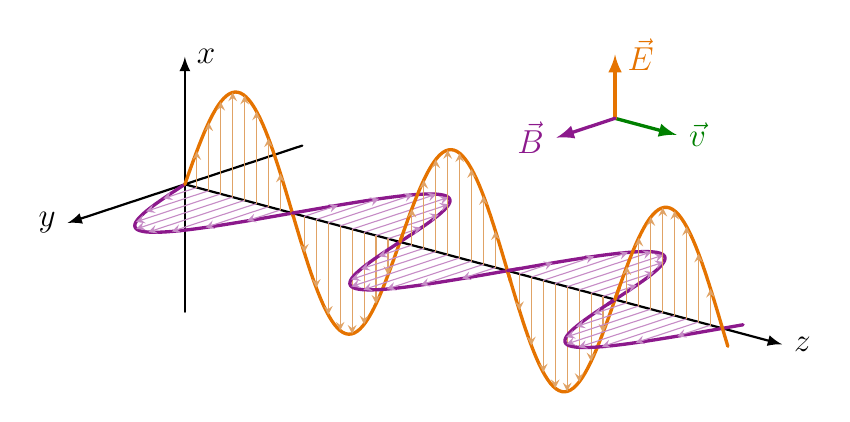
\begin{tikzpicture}[x=(-15:0.9), y=(90:0.9), z=(-150:1.1),
		line cap=round, line join=round,
		axis/.style={black, thick,->},
		vector/.style={>=stealth,->}]
		\large
		\def\A{1.5}
		\def\nNodes{5} % use even number
		\def\nVectorsPerNode{8}
		\def\N{\nNodes*40}
		\def\xmax{\nNodes*pi/2*1.01}
		\pgfmathsetmacro\nVectors{(\nVectorsPerNode+1)*\nNodes}
		\def\vE{{\color{Ecol}\mathbf{E}}}
		\def\vB{{\color{Bcol}\mathbf{B}}}
		
		\def\drawENode{ % draw E node and vectors with some offset
			\draw[Ecol,very thick,variable=\t,domain=\iOffset*pi/2:(\iOffset+1)*pi/2*1.01,samples=40]
			plot (\t,{\A*sin(\t*360/pi)},0);
			\foreach \k [evaluate={\t=\k*pi/2/(\nVectorsPerNode+1);
				\angle=\k*90/(\nVectorsPerNode+1);}]
			in {1,...,\nVectorsPerNode}{
				\draw[vector,EVcol]  (\iOffset*pi/2+\t,0,0) -- ++(0,{\A*sin(2*\angle+\iOffset*180)},0);
			}
		}
		\def\drawBNode{ % draw B node and vectors with some offset
			\draw[Bcol,very thick,variable=\t,domain=\iOffset*pi/2:(\iOffset+1)*pi/2*1.01,samples=40]
			plot (\t,0,{\A*sin(\t*360/pi)});
			\foreach \k [evaluate={\t=\k*pi/2/(\nVectorsPerNode+1);
				\angle=\k*90/(\nVectorsPerNode+1);}]
			in {1,...,\nVectorsPerNode}{
				\draw[vector,Bcol!50]  (\iOffset*pi/2+\t,0,0) -- ++(0,0,{\A*sin(2*\angle+\iOffset*180)});
			}
		}
		
		% MAIN AXES
		\draw[axis] (0,0,0) -- ++(\xmax*1.1,0,0) node[right] {$z$};
		\draw[axis] (0,-\A*1.2,0) -- (0,\A*1.2,0) node[right] {$x$};
		\draw[axis] (0,0,-\A*1.2) -- (0,0,\A*1.2) node[left] {$y$};
		
		% SMALL AXES
		\def\xOffset{{(\nNodes-2)*pi/2}}
		\def\yOffset{\A*1.1}
		\def\zOffset{\A*1.1}
		\draw[axis,very thick,vcol] (\xOffset,\yOffset,-\zOffset) -- ++(\A*0.6,0,0) node[right,align=center] {$\vec{v}$}; %\\propagation
		\draw[axis,very thick,Ecol]  (\xOffset,\yOffset,-\zOffset) -- ++(0,\A*0.6,0) node[right] {$\vec{E}$};
		\draw[axis,very thick,Bcol]   (\xOffset,\yOffset,-\zOffset) -- ++(0,0,\A*0.6) node[left] {$\vec{B}$};
		
		% draw (anti-)nodes
		\foreach \iNode [evaluate={\iOffset=\iNode-1;}] in {1,...,\nNodes}{
			\ifodd\iNode \drawBNode \drawENode % E overlaps B
			\else        \drawENode \drawBNode % B overlaps E
			\fi
		}
	\end{tikzpicture}
	\caption{Elektromagnetische Welle im Vakuum}
	\label{maxwell:section:bild_em_welle}
\end{figure}
In einem luftleeren Raum, in welchem keine Stromdichte $\vec{\jmath}$ und keine Ladungsdichte $\varrho$ existieren, gilt
\begin{align}
\nabla \times \vec{B}
&=
\varepsilon_0\,\mu_0 \frac{\partial \vec{E}}{\partial t}
\label{maxwell:section:ampere_vakuum}
\\
\nabla \times \vec{E}
&=
-\frac{\partial \vec{B}}{\partial t}.
\label{maxwell:section:faraday_vakuum}
\end{align}
Nun können wir in Gleichung \eqref{maxwell:section:ampere_vakuum} die Rotation auf beiden Seiten anwenden und mithilfe der Grassmann-Identität resultiert
\begin{align*}
\nabla \times \nabla \times \vec{B}
&=
\varepsilon_0\,\mu_0 \frac{\partial}{\partial t} (\nabla \times \vec{E})\\
\Leftrightarrow \qquad \nabla \underbrace{(\nabla \cdot \vec{B})}_{\displaystyle=0} - \Delta \vec{B}
&=
-\varepsilon_0\,\mu_0 \frac{\partial ^2 \vec{B}}{\partial t^2}\\
\Leftrightarrow \qquad \frac{\partial ^2 \vec{B}}{\partial t^2}
&=
\underbrace{\frac{1}{\varepsilon_0\,\mu_0}}_{\displaystyle=c^2} \Delta \vec{B}.
\end{align*}
Dies entspricht genau der Wellengleichung.
Mit dem gleichen Vorgehen resultiert für die Gleichung \eqref{maxwell:section:faraday_vakuum}
\begin{align*}
\nabla \times \nabla \times \vec{E}
&=
- \frac{\partial}{\partial t} (\nabla \times \vec{B})\\
\Leftrightarrow \qquad \nabla \underbrace{(\nabla \cdot \vec{E})}_{\displaystyle=0} - \Delta \vec{E}
&=
- \varepsilon_0\,\mu_0 \frac{\partial ^2 \vec{E}}{\partial t^2}\\
\Leftrightarrow \qquad \frac{\partial ^2 \vec{E}}{\partial t^2}
&=
\underbrace{\frac{1}{\varepsilon_0\,\mu_0}}_{\displaystyle=c^2} \Delta \vec{E}.
\end{align*}
Wir kommen also zum Schluss, dass beide Felder die Wellengleichung im genannten Raum erfüllen. Eine Lösung der Wellengleichung kann wie in Abbildung \ref{maxwell:section:bild_em_welle} aussehen. Was dabei auffällt ist, dass die Ausbreitungsgeschwindigkeit in beiden Fällen die Lichtgeschwindigkeit $c$ ist. Daraus kann man schliessen, dass Licht eine elektromagnetische Welle ist.



